%\begin{problem}{\textbf{\textsc{A Tired Flappy Bird}}} A \href{https://flappybird.io/}{flappy bird} can jump multiple times in the air. Each time it jumps mid-air, it can suddenly change its speed and direction. For every jump, the bird can decide when to jump and in which direction. Between jumps, the bird falls freely under gravity, which pulls it down at the acceleration $g$. Say, our tired flappy bird starts off the cliff of height $H$ with the jumping velocity $V[1]=V_0$. Subsequent jumps in mid-air have decreasing velocities, i.e. the $n$-th jump has speed $V[n]=V_0/n$ ($n>1$). This majestic Vietnamese animal wants to travel as far as possible horizontally before it lands on the ground. Find the maximum horizontal distance the bird can travel (denoted as $L$ in the figure below) in meters, given that $H=100$m and $V_0=10$m/s. \textit{Note that each jumping velocity is the total speed of the bird after the jump (rather than e.g. adding to its speed before the jump).}

%\FloatBarrier
%\begin{figure*}[!htbp]
%\centering
%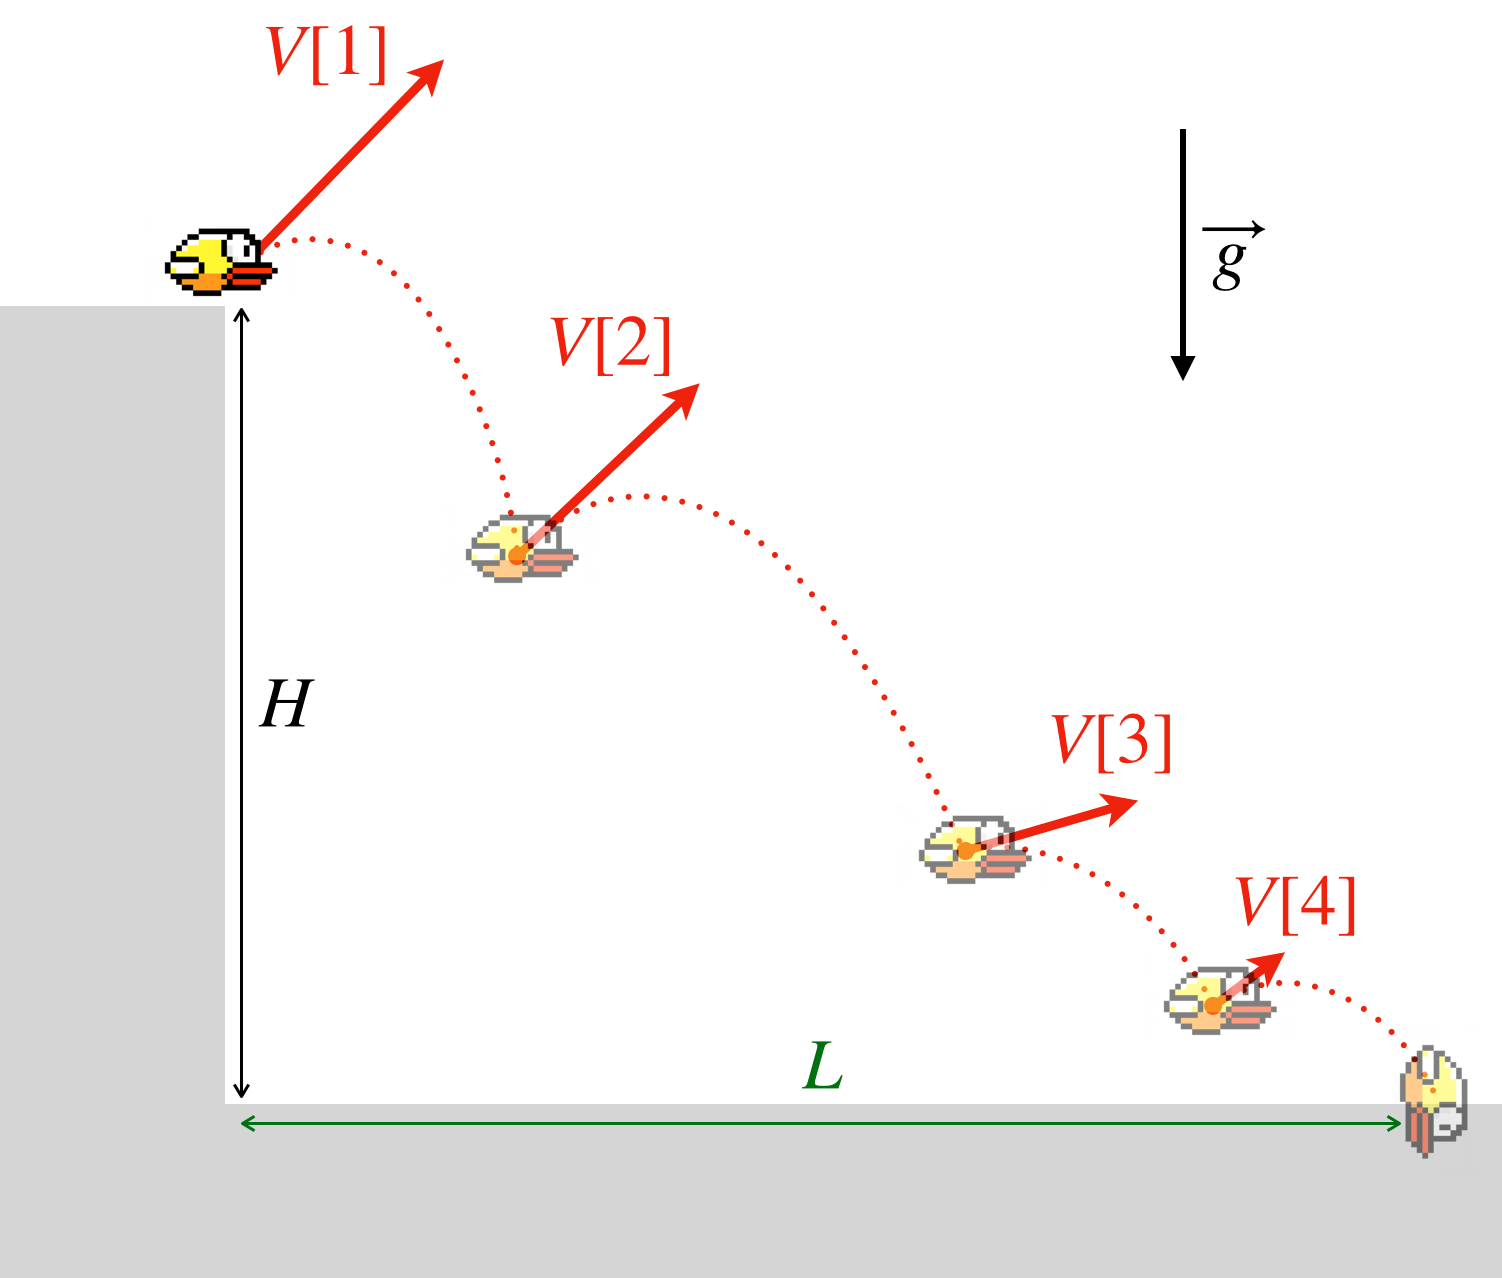
\includegraphics[width=0.5\textwidth]{problems/figures/flappybird.png}
%\end{figure*}
%\FloatBarrier

%\end{problem}

\begin{problem}{\textbf{\textsc{Thứ Flappy Bird mệt mỏi}}} Một chú chim \href{https://flappybird.io/}{flappy bird} có thể nhảy nhiều lần khi đang bay. Mỗi lần nhảy, nó có thể thay đổi tốc độ và hướng đột ngột. Trong mỗi lần nhảy, chú chim có thể quyết định thời điểm nhảy và hướng nhảy. Giữa các lần nhảy, chú chim rơi tự do dưới tác dụng của trọng lực với gia tốc $g$. Giả sử chú chim bắt đầu từ vách đá cao $H$ với vận tốc nhảy ban đầu $V[1]=V_0$. Trong mỗi cú nhảy tiếp theo giữa không trung, vận tốc giảm dần, tức là cú nhảy thứ $n$ có vận tốc $V[n]=V_0/n$ ($n>1$). Con vật dựa trên hình tượng Việt Nam oai hùng này muốn di chuyển xa nhất có thể theo phương ngang trước khi chạm đất. Hãy tìm khoảng cách ngang tối đa mà nó có thể di chuyển (kí hiệu là $L$ trong hình bên dưới) tính bằng mét, biết rằng $H=100$m và $V_0=10$m/s. \textit{Lưu ý rằng mỗi vận tốc sau cú nhảy là vận tốc tổng của con vật sau khi nhảy (thay vì ví dụ như cộng thêm vào vận tốc trước cú nhảy).}
	
	\FloatBarrier
	\begin{figure*}[!htbp]
		\centering
		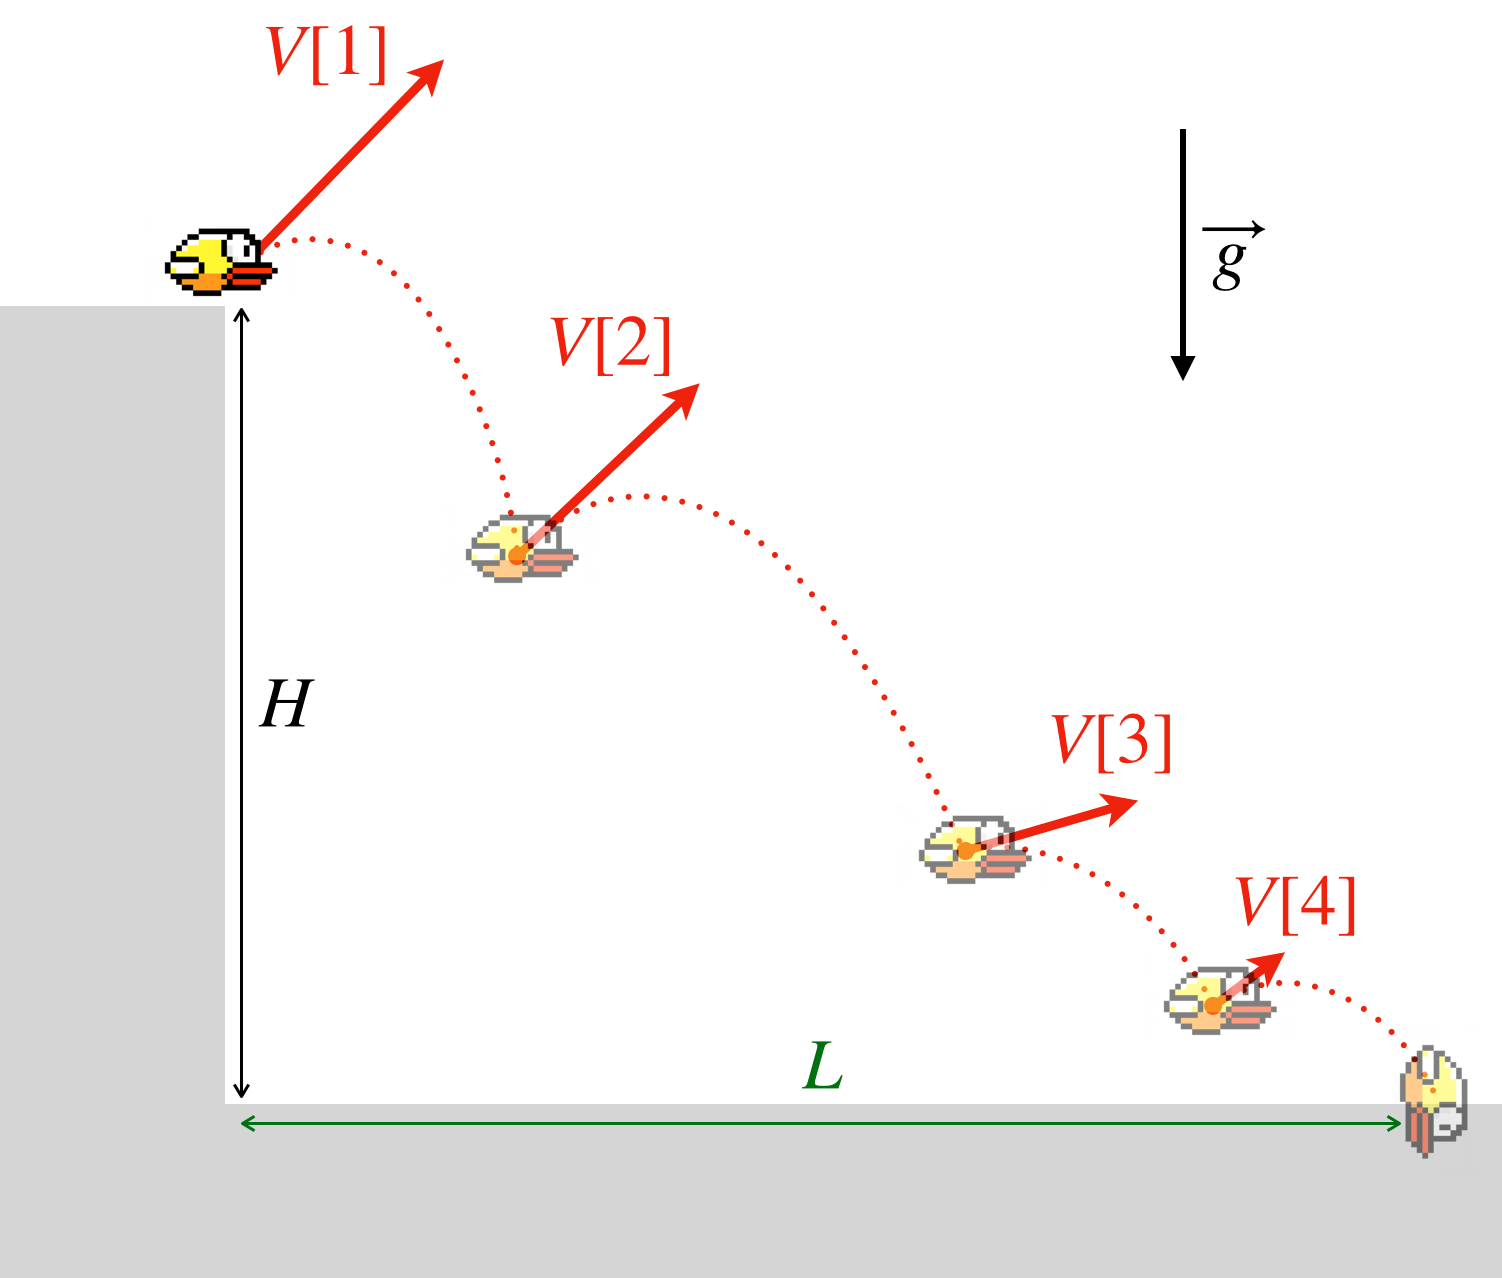
\includegraphics[width=0.5\textwidth]{problems/figures/flappybird.png}
	\end{figure*}
	\FloatBarrier
	
\end{problem}
